\NeedsTeXFormat{LaTeX2e}
\documentclass{jfp}
\usepackage{xcolor}

\title{Composable data visualizations}
\author[Tomas Petricek]{TOMAS PETRICEK\\
       University of Kent, UK\\
       \email{t.petricek@kent.ac.uk}}

\definecolor{kvdclr}{rgb}{0.5,0.0,0.5}
\definecolor{fkvdclr}{rgb}{0.0,0.0,0.6}
\definecolor{urlclr}{rgb}{0.0,0.0,0.8}
\definecolor{idclr}{rgb}{0.0,0.0,0.0}
\definecolor{numclr}{rgb}{0.0,0.4,0.0}
\definecolor{strclr}{rgb}{0.6,0.2,0.0}

\newcommand{\lsep}{\;\;|\;\;}
\newcommand{\num}[1]{\textcolor{numclr}{#1}}
\newcommand{\str}[1]{\textnormal{\textcolor{strclr}{\sffamily "#1"}}}
\newcommand{\strf}[1]{\textnormal{\textcolor{strclr}{\sffamily #1}}}
\newcommand{\ident}[1]{\textnormal{\textcolor{idclr}{\sffamily #1}}}
\newcommand{\kvd}[1]{\textnormal{\textcolor{kvdclr}{\sffamily #1}}}
\newcommand{\fkvd}[1]{\textnormal{\textcolor{fkvdclr}{\sffamily #1}}}
\newcommand{\narrow}[1]{\hspace{-0.6em}#1\hspace{-0.6em}}
\newcommand{\urrl}[1]{\textnormal{\textcolor{urlclr}{\url{#1}}}}
\begin{document}
\maketitle[f]

% \begin{abstract}
% This guide is for authors who are preparing papers for the \emph{Journal of
% Functional Programming} using the \LaTeXe\ document-preparation system
% and the Functional Programming class file (\texttt{jfp1.cls}).
% \end{abstract}


\bibliographystyle{jfp}

\section{Introduction}
Let's say we want to create the two charts in Figure~\ref{fig:charts}. The chart on the left is
a bar chart that shows two different values for each bar. The chart on the right consists of two
line charts that share the X axis and highlight two parts of the timeline with two different colors.

There is a plenty of libraries that can draw bar charts and line charts, but adding those extra
features will only be possible if the author already thought about your exact scenario. For
example, Google Charts supports the left chart (it is called Dual-X Bar Chart) but there is no
way for adding a background, or sharing an axis between charts. The alternative is to use a more
low-level library such as D3. In D3 you construct the chart piece by piece, but then you have to
tediously transform your values to coordinates in pixels yourself. For scientific plots,
you could use an implementation of Grammar of Graphics such as ggplot2, where a chart is
a mapping from data to geometric objects (such as points, bars, and lines) and their visual
properties (X and Y coordinate, shape and color). However, the range of charts that can be
created using this systematic approach is still somewhat limited.

What would an elegant functional approach to data visualization look like? A functional programmer
would want a domain-specific language that has a small number of primitives; allow us to define
high level abstractions such as a bar chart and its basic building blocks are expressed in terms
of domain values such as the exchange rate, rather than pixels.

\begin{figure}[h]
  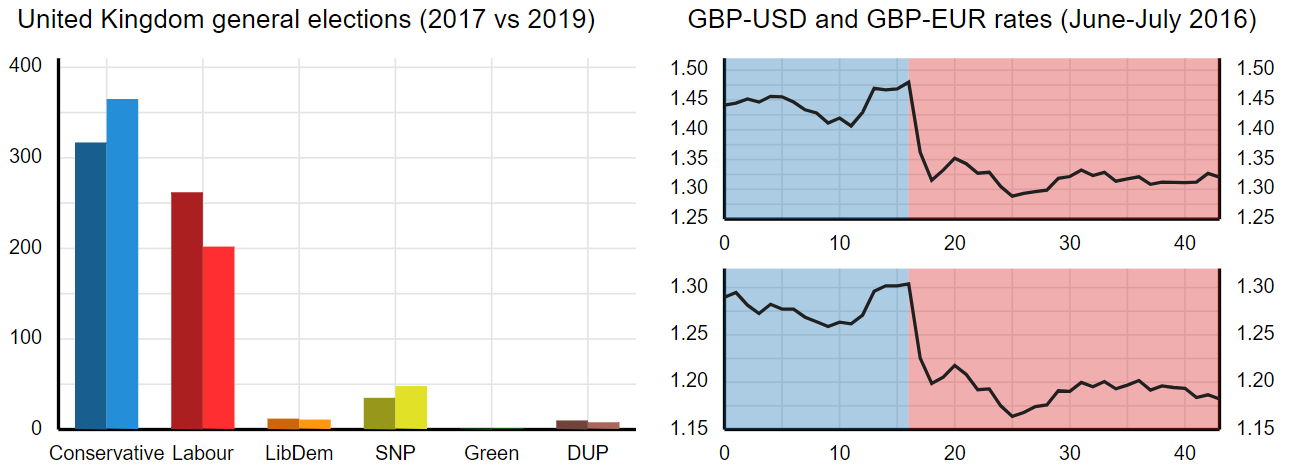
\includegraphics[scale=0.57]{figures/charts}
  \vspace{0.25em}
  \caption{Two charts about the UK politics: Comparison of election results from 2017 and 2019 (left)
    and GBP-USD exchange rate with highlighted areas before and after the 23 June 2016 Brexit vote.}
  \label{fig:charts}
\end{figure}

As is often the case with domain-specific languages, finding the right primitives is more of an art
than science. For this reason, I present my answer -- a library named Compost -- as a functional pearl.
I hope to convince the reader that Compost is elegant and I illustrate this with a wide range
of examples. Compost has a number of specific desirable properties:

\begin{itemize}
\item Charts are composed from a small number of primitive building blocks using a small number of
  combinators. In particular, concepts such as bar charts, line charts or charts with aligned
  axes are expressed in terms of more basic concepts.
\item The primitives are specified in domain terms. When drawing a line, the value of an Y coordinate
  is an exchange rate of 1.36 USD/GBP, not 137 pixels from the bottom.
\item Most common chart types can be easily captured as high level abstractions, but there is an
  elengant way of creating a majority of more interesting custom charts.
\item The approach can easily be extended to creating web-based charts that involve animations
  or interaction with the user.
\end{itemize}
%
The presentation in this paper focuses on explaining the primitives and combinators of the
domain-specific language. I outline the structure of an implementation, but omit the details. Filling
those in requires careful thinking about geometry and projections, but there are no unexpected
surprises. A complete F\# implementation, including the examples used in this paper, is available
at: \urrl{http://github.com/compostjs}.

\section{Basic charts: Overlaying chart primitives}
I will introduce individual features of the Compost library gradually. The first important aspect of
Compost is that properties of shapes are defined in terms of domain-specific values. I first
explain what this means and then use domain-specific values to specify the core part of the
UK election results bar chart.

\begin{figure}[t]
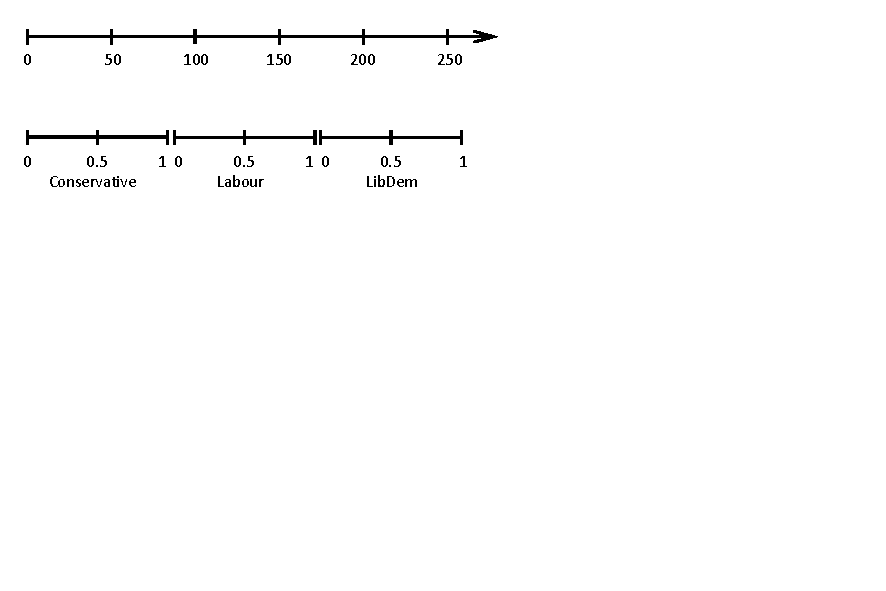
\includegraphics[scale=1,trim={0cm 6.5cm 6cm 0cm},clip]{figures/values.pdf}
\caption{On a continuous scale (above), an exact position is determined by a number.
  On a categorical scale (below), an exact position is determined by the category and a
  numerical ratio from 0 to 1.}
\label{fig:scales}
\end{figure}

\subsection{Domain-specific values}

In the election results chart in Figure~\ref{fig:charts} (left), the X values are categorical
values representing the political parties such as \strf{Conservative} or \strf{Labour}. The
Y values are numerical values representing the number of seats won such as $\num{365}$ MPs.
When creating data visualizations, those are the values that the user needs to specify. This is
akin to most high-level charting libraries such as Google Charts, but in contrast with more
flexible libraries like D3.

Our design focuses on two-dimensional charts with X and Y axes. Values mapped to those axes
can be either categorical (such as different political parties or countries) or continuous
(such as number of votes or exchange rates). The mapping from categorical and continuous values
to exact positions on the chart is done automatically. For continuous values, this simply means
applying a linear transformation. For categorical values, the mapping is more difficult.

For example, in the UK election results chart, the X axis is categorical. The library automatically
divides the available space between the six categorical values (political parties). The value
\strf{Green} does not determine an exact position on the axis, but rather a range. To determine
an exact position, we also need to attach a value between $\num{0}$ and $\num{1}$ to the
categorical value. This identifies a relative position in the available range.

Figure~\ref{fig:scales} illustrates the two kinds of values using the axes from the UK
election results chart. In Figure~\ref{fig:shape}, we define a value $v$ as either a continuous value
$\kvd{cont}~n$ containing any number $n$ or a categorical value $\kvd{cat}~c, r$, consisting
of a categorical value $c$ (implemented as a string) and a ratio $r$ between $0$ and $1$.
%
\begin{figure}
\begin{equation*}
\begin{array}{rcl}
v & = & \kvd{cat}~c, r \\
  & | & \kvd{cont}~n\\
  ~
\end{array}
\qquad
\begin{array}{rclcl}
s & = &\kvd{line}~\gamma, [\,v_{x1}, v_{y1}, \ldots, v_{xn}, v_{yn}\,] & | & \kvd{overlay}~[\,s_1, \ldots, s_n\,]\\
 & | & \kvd{fill}~\gamma, [\,v_{x1}, v_{y1}, \ldots, v_{xn}, v_{yn}\,] & | &\kvd{axis}_{l/r/t/b}~s\\
 & | & \kvd{text}~\gamma, v_x, v_y, t & | &\kvd{padding}~n_t,n_r,n_b,n_l,s
\end{array}
\end{equation*}
\caption{Core primitives of the Compost domain-specific language. Values $v$ are either categorical
  or continuous; a shape $s$ is then defined as a simple recursive algebraic data type.}
\label{fig:shape}
\end{figure}

\subsection{Basic primitives and combinators}

Now that we know how Compost represents values, we can define the basic elements of its
domain-specific langauge. A chart is represeted by the shape $s$ defined in Figure~\ref{fig:shape}.
A primitive shape can be a text label, a line connecting a list of points or a filled polygon
defined by a list of points. The position of points is specified by X and Y coordinates,
which can be either categorical or continuous values. For text, line and polygon, we also include
a parameter $\gamma$ that specifies the element color.

Figure~\ref{fig:shape} also defines three combinators. The most important is $\kvd{overlay}$,
which overlays all shapes from a given list. When doing this, Compost automatically infers the
scales of X and Y axes and calculates suitable projections using a method discussed in the next
section. Finally, $\kvd{padding}$ adds padding around a specified shape and $\kvd{axis}$ adds
an axis showing the inferred scale on the left, right, top or bottom of a given shape.
Using those primitives, we can construct the simple UK election results bar chart in Figure~\ref{fig:simple} (left).
We use the \fkvd{let} construct of the host functional language to structure the code:
%
\begin{equation*}
\begin{array}{l}
\fkvd{let}~\ident{conservative},~\ident{labour}~=\\
\quad \kvd{fill}~\strf{\#0000ff},
 ~[\;\,(\kvd{cat}~\strf{Conservative}, \num{0}), (\kvd{cont}~\num{0}), (\kvd{cat}~\strf{Conservative}, \num{0}), (\kvd{cont}~\num{365}),\\
\hspace{6.7em}\;(\kvd{cat}~\strf{Conservative}, \num{1}), (\kvd{cont}~\num{365}), (\kvd{cat}~\strf{Conservative}, \num{1}), (\kvd{cont}~\num{0})\;\,],\\
\quad \kvd{fill}~\strf{\#ff0000},
 ~[\;\,(\kvd{cat}~\strf{Labour}, \num{0}), (\kvd{cont}~\num{0}), (\kvd{cat}~\strf{Labour}, \num{0}), (\kvd{cont}~\num{202}),\\
\hspace{6.7em}\;(\kvd{cat}~\strf{Labour}, \num{1}), (\kvd{cont}~\num{202}), (\kvd{cat}~\strf{Labour}, \num{1}), (\kvd{cont}~\num{0})\,\;]\\[0.5em]
\kvd{axis}_l~(\kvd{axis}_b~(\kvd{overlay}~[~\ident{labour}, \ident{conservative}~]))\\
\end{array}
\end{equation*}

\noindent
The chart specification overlays two bars of different colors and then adds axes to the bottom and
left of the chart. The two bars are filled rectangles defined using four corner points. The Y
coordinates are specified as continuous values, while the X coordinates are categorical. For
the Conservative party, two of the points have the Y coordinate set to $\kvd{cont}~\num{0}$ (bottom of the bar)
and two have the Y coordinate set to $\kvd{cont}~\num{365}$ (top of the bar). The two X coordinates
are the start and the end of the range allocated for the \strf{Conservative} category,
i.e.~$\kvd{cat}~\strf{Conservative}, \num{0}$ on the left and $\kvd{cat}~\strf{Conservative}, \num{1}$
on the right.

\begin{figure}
  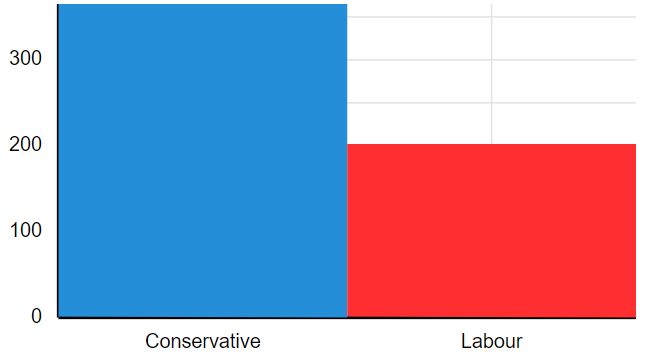
\includegraphics[scale=0.57]{figures/simple}
  \vspace{0.25em}
  \caption{Simple chart showing the UK election results; using automatically inferred scales (left)
    and using rounded Y scale and explicitly defined (reordered) X scale (right).}
  \label{fig:simple}
\end{figure}

Extending the snippet to generate a grouped bar chart that shows two results
for each party as in Figure~\ref{fig:charts} is easy. Given a party $p$, we need to
generate two rectangles, one with X coordinates $\kvd{cat}~p, 0$ and $\kvd{cat}~p, 0.5$
and the other with X coordinates $\kvd{cat}~p, 0.5$ and $\kvd{cat}~p, 1$.
In the following snippet, we use a \fkvd{for} comprehension to generate the list. All remaining
constructs are primitives of the Compost domain-specific language. Assuming \ident{elections} is a
list of election results containing a five-element tuple consisting of a party name, colors for
2017 and 2019 and results for 2017 and 2019 we create the chart using:
%
\begin{equation*}
\begin{array}{l}
  \kvd{axis}_l~(\kvd{axis}_b~(\kvd{overlay}~[\\
  \quad \fkvd{for}~\ident{party}, \ident{clr17}, \ident{clr19}, \ident{mp17}, \ident{mp19}~\fkvd{in}~\ident{elections}~\rightarrow\\
  \quad\quad \kvd{padding}~0,10,0,10,\,\kvd{overlay}~[\\
  \quad\quad\quad \kvd{fill}~\ident{clr17},~[\,(\kvd{cat}~\ident{party}, \num{0}), (\kvd{cont}~\num{0}), (\kvd{cat}~\ident{party}, \num{0}), (\kvd{cont}~\ident{mp17}),\\
  \quad\quad\quad \hspace{4.08em}           ~(\kvd{cat}~\ident{party}, \num{0.5}), (\kvd{cont}~\ident{mp17}), (\kvd{cat}~\ident{party}, \num{0.5}), (\kvd{cont}~\num{0}) \,], \\
  \quad\quad\quad \kvd{fill}~\ident{clr19},~[\,(\kvd{cat}~\ident{party}, \num{0.5}), (\kvd{cont}~\num{0}), (\kvd{cat}~\ident{party}, \num{0.5}), (\kvd{cont}~\ident{mp19}),\\
  \quad\quad\quad \hspace{4.08em}           ~(\kvd{cat}~\ident{party}, \num{1}), (\kvd{cont}~\ident{mp19}), (\kvd{cat}~\ident{party}, \num{1}), (\kvd{cont}~\num{0})\,]~~]~~]\,)\,)\\
\end{array}
\end{equation*}

\noindent
Aside from iterating over all available parties and splitting the bar, the example also adds padding
around the bars. A padding is specified in pixels rather than in terms of domain values. This is
sometimes preferrable over, for example, drawing a bar using a range from $\num{0.05}$ to $\num{0.5}$.
One remaining feature of the chart in Figure~\ref{fig:charts} that is still missing is the caption.
We will add this in Section~\ref{sec:abstractions}.

\subsection{Inferring scales and projections}

When composing shapes using the \kvd{overlay} primitive, the user does not need to specify how
to position the child elements relatively to each other. The Compost library positions the elements
automatically. This is done in two steps. First, Compost infers the \emph{scales} for X and Y
axes. A scale represents the range of values that needs to fit in the space available for the chart.
Second, Compost calculates a \emph{projection}, a mapping from domain-specific values of the scale
to the available screen space. A scale $l$ is defined in Figure~\ref{fig:scale}.

\begin{figure}
\vspace{-0.5em}
\begin{equation*}
\begin{array}{rcl}
l & = & \kvd{continuous}~n_{min}, n_{max} \lsep \kvd{categorical}~[\,c_1, \ldots, c_k\,]
\end{array}
\end{equation*}
\vspace{-1em}
\caption{A scale $l$ can be continuous, defined by a range, or categorical, defined by a list of values.}
\label{fig:scale}
\vspace{-1em}
\end{figure}
\begin{figure}
\begin{equation*}
\begin{array}{rclcl}
s & = & \kvd{roundScale}_{x/y} s      &|& \kvd{nest}_{x/y}~v_{min}, v_{max}, s \\
  & | & \kvd{explicitScale}_{x/y}~l, s &|&  (\ldots)
\end{array}
\end{equation*}
\vspace{-0.5em}
\caption{Additional combinators for controlling and nesting scales, extending earlier definition of $s$.}
\label{fig:control}
\end{figure}

A continuous scale is defined by a minimal and maximal value that need to be mapped to the
available chart space. A categorical scale is defined by a list of individual categorical values.
Note that we do not need a minimal and maximal ratios of the used categorical values as Compost
will use an equal space for each category, regardless of where in this space a shape needs to
appear.

Inferring scales is done by a simple recursive function that walks over the given shape and
constructs two scales for the X and Y axis, using the X and Y coordinates that appear in the shape.
Most of the work is done by a simple helper function that takes two scales, $l_1$ and $l_2$,
and produces a new scale that represents the union of the two:
%
\begin{equation*}
\begin{array}{l}
\ident{union}~(\kvd{continuous}~n_l, n_h)~(\kvd{continuous}~n'_l, n'_h) =\\
\qquad\kvd{continuous}~\min(n_l, n'_l), \max(n_h, n'_h)\\[0.5em]
\ident{union}~(\kvd{categorical}~[\,c_1, \ldots, c_p\,])~(\kvd{categorical}~[\,c'_1, \ldots, c'_q\,]) =\\
\qquad \kvd{categorical}~[\,c_1, \ldots, c_p\,] \;@\; [\,c'_i~|~ \forall i\in 1\ldots q, \nexists j. c_j = c'_i \;]
\end{array}
\end{equation*}

\vspace{-0.5em}
\noindent
When unioning two continuous scales, the minimum and maximum of the resulting scale is the smallest
and largest of the two minimums and maximums, respectively. When unioning two categorical scales,
we take all values of the first scale and append all values of the second scale that do not appear
in the first one. Note that this means that the order of categorical values in a scale depends on
the order in which they appear in the shape. (A possible improvement to Compost would be to support
ordinal values, which are categorical values with a well-defined ordering.) It is also worth noting
that a categorical scale cannot be combined with a continuous scale. In other words, mixing
categorical and continuous values in a single scale results in an error.

Once Compost computes scales for a given shape and its sub-shapes, it constructs a projection
that maps domain-specific values to the available chart space. We discuss this in
Section~\ref{sec:impl}. For a continuous scale, the projection is a linear transformation. For
categorical scale with $k$ values, we split the available chart space into $k$ equally sized
regions and then map a categorical value $\kvd{cat}~c, r$ to the region corresponding to $c$
according to the ratio $r$.

\section{Advanced charts: Controlling scale composition}
\label{sec:fancy}

Most charts have one X and one Y axis that are determined by the values the chart shows,
but there are interesting exceptions. The chart in Figure~\ref{fig:charts} (right)
has two different Y axes, one for GBP-USD and one for GBP-EUR. In the next two sections, we look at
three combinators that control the scale inferrence process and what flexibility this enables.

\subsection{Defining nice scale ranges}

The automatic scale inference often results in scales where the maximum is a non-round number.
This leads to charts that fully utilize the available space, but may not be easy to read.
The first two primitives, shown in Figure~\ref{fig:control} (left) allow the chart designer
to adjust the automatically inferred range of scales.

The two combinators for controlling the range of scales are \kvd{roundScale} and \kvd{explicitScale}.
The oprations can be applied to either the X scale or the Y scale, which is indicated by the
$x/y$ sub-script. The \kvd{roundScale} primitve takes the inferred X or Y scale of the shape $s$
and, if it is a continuous scale, rounds its minimal and maximal values to a ``nice'' number.
For example, if a continuous scale has minimum $\num{0}$ and maximum $\num{365}$, the resulting
scale would have a maximum $\num{400}$. For categorical scale, the operation does not have any effect.
The \kvd{explicitScale} operation is similar, but it replaces the inferred scale with an explicitly
provided scale (the type of the inferred scale has to match with the type of the explicitly given
scale). For example, the chart in Figure~\ref{fig:simple} (right) is constructed using the
following code (reusing the \ident{labour} and \ident{conservative} variables defined earlier):
%
\begin{equation*}
\begin{array}{l}
\kvd{axis}_l~(\kvd{axis}_b~(\kvd{roundScale}_y~(\kvd{explicitScale}_x~(\kvd{categorical}~[\,\strf{Labour},\strf{Conservative}\,]),\\
\qquad \kvd{overlay}~[~\ident{labour}, \ident{conservative}~]~)))\\
\end{array}
\end{equation*}
\vspace{-0.5em}

\noindent
Reading the code from the inside out, the snippet first overlays the two coloured bars defined
earlier; it then replaces the X axis with an explicitly given one that changes the order of the
values. As a result, the bar for \strf{Labour} will appear on the left, even though the value
comes later in the list of overlaid chart elements.

The code next uses \kvd{roundScale} to automatically round the minimum and maximum of the
continuous Y scale (showing the total number of seats). Finally, we add axes around the shape,
producing a usual labelled chart.  It is worth noting that \kvd{axis} and \kvd{roundScale}
could be implemented as derived operations; \kvd{roundScale} would need to infer the scale of
the nested shape and then insert \kvd{explicitScale} with a rounded number; \kvd{axis}
would also need to infer the scales and then generates labels and lines in suitable locations.

\begin{figure}
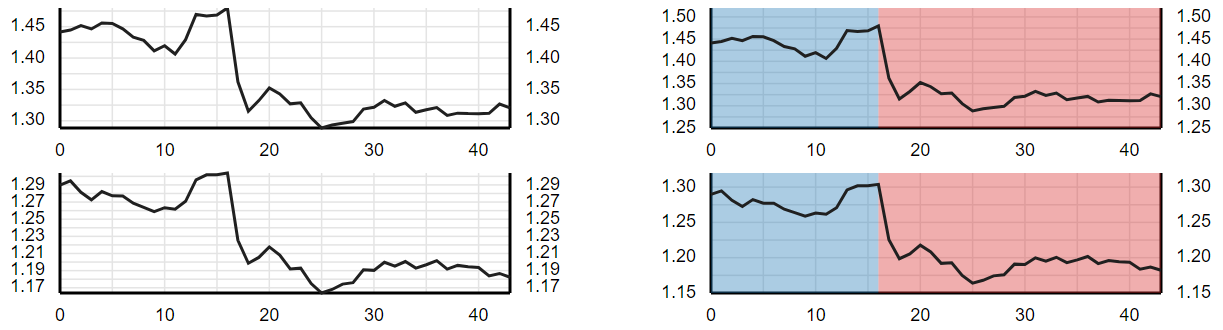
\includegraphics[scale=0.57]{figures/lines}
\vspace{0.25em}
\caption{Two charts showing currency exchange rates with a shared X scale and separate Y scales.}
\label{fig:lines}
\end{figure}

\subsection{Nested scales}

The most interesting primitive for controlling scale composition defined in Figure~\ref{fig:control}
is $\kvd{nest}_{x/y}$. The combinator takes two values, $v_{min}, v_{max}$ and a shape $s$ as arguments
and it nests the scale of the shape $s$ inside the region defined by $v_{min}, v_{max}$. When inferring
scales of shapes, the scale of $\kvd{nest}_{x/y}~l, s$ will be a categorical or continuous scale
inferred using the values $v_{min}$ and $v_{max}$, regardless of the values that are used inside
the shape $s$. The chart space between $v_{max}$ and $v_{min}$ will then be used to render the
nested shape $s$ using its inferred scale. An example of nesting is shown in Figure~\ref{fig:nesting}.
Here, a chart with a continous scale from $\num{1.1}$ to $\num{1.4}$ (e.g.~GBP-EUR exchange rates)
is nested in the left half of another chart, which has a continuous scale from $\num{0}$ to $\num{100}$.

\begin{figure}
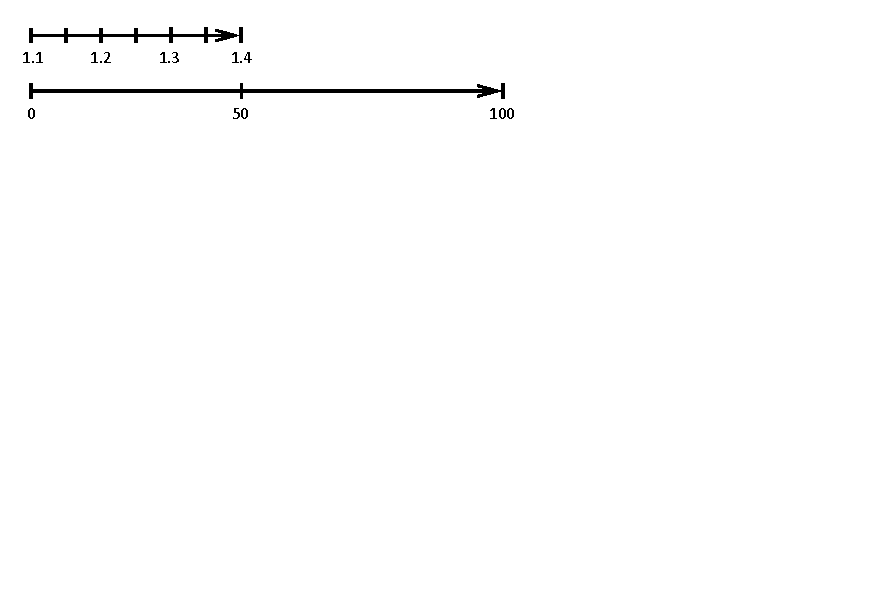
\includegraphics[scale=1,trim={0cm 7.5cm 6cm 0cm},clip]{figures/nest}
\caption{A continuous scale with values from $0$ to $6$, nested in another scale.}
\label{fig:nesting}
\end{figure}

The nesting of scales can be used in a variety of ways. We can, for example, nest a line chart
inside a bar of a bar chart. In that case, the values for $v_{min}$ and $v_{max}$ would be
$\kvd{cat}~\strf{ABC}, 0$ and $\kvd{cat}~\strf{ABC}, 1$, which define the start and the end of
the region allocated to the $\strf{ABC}$ category on a categorical scale. A simpler use case for
the combinator is showing multiple charts in a single view. For example, the motivating example
in Figure~\ref{fig:charts} (right) comapres aligned line charts of exchange rates for two
different currencies. Assuming \ident{gbpusd} and \ident{gbpeur} are lists containing days as X
values and exchange rates as Y values, we can construct a simple chart with two line charts,
shown in Figure~\ref{fig:lines} (left), using:
%
\begin{equation*}
\begin{array}{l}
\kvd{overlay}~[~
\kvd{nest}_y~(\kvd{cont}~\num{0}),(\kvd{cont}~\num{50}), (\kvd{axis}_l~(\kvd{axis}_r~(\kvd{axis}_b~(\kvd{line}~\strf{\#202020}~\ident{gbpusd}))))\\
\hspace{3.68em} \kvd{nest}_y~(\kvd{cont}~\num{50}),(\kvd{cont}~\num{100}), (\kvd{axis}_l~(\kvd{axis}_r~(\kvd{axis}_b~(\kvd{line}~\strf{\#202020}~\ident{gbpeur}))))~]\\
\end{array}
\end{equation*}

\vspace{-0.5em}
\noindent
In this example, the X scale shows the days of the year. This scale is shared by both of the charts.
Indeed, if data was only available for the second half of the month for one of the charts,
we would want the line to start in the middle of the chart. However, the Y scale needs to be
separate for each of the charts. To achieve this, we use $\kvd{nest}_y$. The scale of the inner
shapes is continuous, from the minimal to the maximal exchange rate for a given period. The
outer scale is determined by the explicitly defined points. For the upper chart, these are
$\kvd{cont}~\num{0}$ and $\kvd{cont}~\num{50}$; for the lower chart, these are
$\kvd{cont}~\num{50}$ and $\kvd{cont}~\num{100}$. The continuous values define a scale that only
contain two shapes -- one in the upper half, one in the lower half -- and so the three numbers could
have equally been, for example, $\num{0},\num{1}, \num{2}$. The outer scale used here is
synthetic and it is not aligned with other chart elements. An example of a more complex chart
that follows a similar style, but does not have synthetic outer scale would be pairplot from
the seaborn Python library. % \cite

For completeness, the following code snippet shows how to construct the full currency exchange
rate chart shown in Figure~\ref{fig:lines} (right), including the blue and red background:
%
\begin{equation*}
\begin{array}{l}
\fkvd{let}~\ident{brexitRate}~(\ident{lo}, \ident{hi})~\ident{rates}~=\kvd{overlay}~[\\
\quad \kvd{fill}~\strf{\#1F77B460}, [\;\,\kvd{cont}~\num{0}, \kvd{cont}~\ident{lo}, \kvd{cont}~\num{16}, \kvd{cont}~\ident{lo}, \kvd{cont}~\num{16}, \kvd{cont}~\ident{hi}, \kvd{cont}~\num{0}, \kvd{cont}~\ident{hi}\;],\\
\quad \kvd{fill}~\strf{\#D6272860}, [\;\,\kvd{cont}~\num{16}, \kvd{cont}~\ident{lo}, \kvd{cont}~\num{44}, \kvd{cont}~\ident{lo}, \kvd{cont}~\num{44}, \kvd{cont}~\ident{hi}, \kvd{cont}~\num{16}, \kvd{cont}~\ident{hi}\;],\\
\quad \kvd{line}~\strf{\#202020}~\ident{rates}~]\\[0.5em]
\kvd{overlay}~[~
\kvd{nest}_y~(\kvd{cont}~\num{0}),(\kvd{cont}~\num{50}), (\kvd{axis}_l~(\kvd{axis}_r~(\kvd{axis}_b~(\ident{brexitRate}~(\num{1.25}, \num{1.50})~\ident{gbpusd}))))\\
\hspace{3.68em} \kvd{nest}_y~(\kvd{cont}~\num{50}),(\kvd{cont}~\num{100}), (\kvd{axis}_l~(\kvd{axis}_r~(\kvd{axis}_b~(\ident{brexitRate}~(\num{1.15}, \num{1.30})~\ident{gbpeur}))))~]\\
\end{array}
\end{equation*}

\noindent
Here, we use the \fkvd{let} binding of the host language to define a function that takes
a the data \ident{rates} together with the minimum and maximum. This is used for drawing
two filled rectangles, covering the first 16 days of the view in blue and the rest in red.
The shapes combined using \kvd{overlay} are rendered in the order in which they appear and so
the line shape is last, so that it appears above the background.

\section{Definining abstractions}
\label{sec:abstractions}

\begin{equation*}
\begin{array}{l}
\fkvd{let}~\ident{title}~t~s~=\ident{overlay}~[\\
\quad \kvd{nest}_x~(\kvd{cont}~\num{0}), (\kvd{cont}~\num{100}),
  (\kvd{nest}_y~(\kvd{cont}~\num{0}), (\kvd{cont}~\num{15}), \\
\quad\quad \kvd{explicitScale}_x~(\kvd{continuous}~\num{0},\num{100}),~(\kvd{explicitScale}_y~(\kvd{continuous}~\num{0},\num{100}),\\
\quad\qquad \kvd{text}~\strf{\#000000}, (\kvd{cont}~\num{50}), (\kvd{cont}~\num{50}),~t)~)\\
\quad \kvd{nest}_x~(\kvd{cont}~\num{0}), (\kvd{cont}~\num{100}),
  (\kvd{nest}_y~(\kvd{cont}~\num{15}), (\kvd{cont}~\num{100}),~s)~]
\end{array}
\end{equation*}

\begin{equation*}
\begin{array}{l}
\fkvd{let}~\ident{pairplot}~\ident{attrs}~\ident{data}~=~\kvd{overlay}~[\\
\quad \kvd{for}~x~\kvd{in}~\ident{attrs}~\rightarrow~\kvd{for}~y~\kvd{in}~\ident{attrs}~\rightarrow\\
\qquad \kvd{nest}_x~(\kvd{cat}~x, 0), (\kvd{cat}~x, 1), (\kvd{nest}_y~(\kvd{cat}~y, 0), (\kvd{cat}~y, 1), \\
\quad\qquad (\kvd{axis}_l~(\kvd{axis}_b~(\kvd{overlay}~[~\fkvd{for}~v~\kvd{in}~\ident{data}~\rightarrow~\kvd{bubble}~(\ident{get}~x~v), (\ident{get}~y~v), \num{1}, \num{1} ])))~)]\\
\end{array}
\end{equation*}

let
  Shape.Layered [
    for x in ["sepal.length"; "sepal.width"; "petal.length"; "petal.width" ] do
      for y in ["sepal.length"; "sepal.width"; "petal.length"; "petal.width" ] do
        yield Shape.OuterScale(Some(Categorical [| ca x |]), Some(Categorical [| ca y |]),
          Shape.Axes(false, false, true, true, Shape.Layered [
            for v, k in iris ->
              Derived.StrokeColor(colors.[k], Shape.Bubble(numv v.[x], numv v.[y], 1., 1.))
          ]))
  ] |> render "out3"



\newpage

\section{Interactive charts}

\section{Implementation structure}
\label{sec:impl}

\newpage


\subsection*{Controlling and nesting scales}


\subsection*{Nesting of charts and scales}

~
~
\noindent
[TODO: We really need illustrations for those example charts, but that would be more work!]
~
[TODO: Maybe use this chart as a motivation: https://wellcomeopenresearch.org/articles/4-63/v1]
~
\section{Random ideas}
\begin{itemize}
\item We could define a type system to catch categorical/continuous value mismatch in a single %scale.
\item It would be worth thinking about ordinal values, which are categorical but can be sorted.
\item There might be other kinds of scales - for example, color scale (can have meaning in scatter plot)
 or a scale for secondary markers (like sizes of bubbles in a bubble chart). We could really say that
 every value (including bar chart colors) should be coming from some scale...
\item Implementing something like \kvd{axis} or \kvd{roundScale} as an actual derived primitive is
 a bit tricky, because it needs to invoke a part of the normal rendering workflow (to run the
 automatic inference of scales on the nested shape) -- this might be just implementation issue,
 but it could be some more basic problem.
\end{itemize}
\end{document}

%


% \usepackage{booktabs}
% \usepackage{subcaption}
% \usepackage{lineno,hyperref,xcolor}
% \usepackage{flushend}
% \usepackage{stmaryrd}
% \usepackage{amssymb}
% \usepackage{xypic}
% \usepackage{semantic}
% \usepackage{booktabs}
% \usepackage{enumitem}
% \usepackage{enumerate}
% \usepackage{amsmath}
% \usepackage[T1]{fontenc}
%
% \setlist{leftmargin=6mm}
% \newcounter{thc}
% \newcounter{dfc}
%
% \theoremstyle{plain}
% \newtheorem{lem}[thc]{Lemma}
% \newtheorem{theorem}[thc]{Theorem}
%
% \theoremstyle{definition}
% \newtheorem{axiom}[dfc]{Axiom}
% \newtheorem{definition}[dfc]{Definition}
%
% \title{Compost: Library for composable data visualization}
% %\author{Tomas Petricek}
% %\affiliation{
% %  \institution{University of Kent}
% %  \country{United Kingdom}
% %}
% %\email{tomas@tomasp.net}
%
% %\begin{CCSXML}
% %<ccs2012>
% %<concept>
% %<concept_id>10011007.10011006.10011008</concept_id>
% %<concept_desc>Software and its engineering~General programming languages</concept_desc>
% %<concept_significance>500</concept_significance>
% %</concept>
% %<concept>
% %<concept_id>10003456.10003457.10003521.10003525</concept_id>
% %<concept_desc>Social and professional topics~History of programming languages</concept_desc>
% %<concept_significance>300</concept_significance>
% %</concept>
% %</ccs2012>
% %\end{CCSXML}
% %
% %\ccsdesc[500]{Software and its engineering~General programming languages}
% %\ccsdesc[300]{Social and professional topics~History of programming languages}
%
% \definecolor{cmtclr}{rgb}{0.0,0.6,0.0}
% \definecolor{kvdclr}{rgb}{0.0,0.0,0.6}
% \definecolor{idclr}{rgb}{0.0,0.0,0.0}
% \definecolor{numclr}{rgb}{0.0,0.4,0.0}
% \definecolor{strclr}{rgb}{0.4,0.4,0.0}
% \definecolor{rstrclr}{rgb}{0.5,0.1,0.0}
% \definecolor{prepclr}{rgb}{0.6,0.0,0.2}
% \newcommand{\vect}[1]{\langl #1 \rangl}
% \newcommand{\langl}{\begin{picture}(4.5,7)
% \put(1.1,2.5){\rotatebox{60}{\line(1,0){5.5}}}
% \put(1.1,2.5){\rotatebox{300}{\line(1,0){5.5}}}
% \end{picture}}
% \newcommand{\rangl}{\begin{picture}(4.5,7)
% \put(.9,2.5){\rotatebox{120}{\line(1,0){5.5}}}
% \put(.9,2.5){\rotatebox{240}{\line(1,0){5.5}}}
% \end{picture}}
% \newcommand{\ball}[1]{\FPeval{\result}{clip(201+#1)}\textnormal{\ding{\result}}}
% \newcommand{\lsep}{\;\;|\;\;}
% \newcommand{\num}[1]{\textcolor{numclr}{#1}}
% \newcommand{\str}[1]{\textnormal{\textcolor{strclr}{\sffamily "#1"}}}
% \newcommand{\strf}[1]{\textnormal{\textcolor{strclr}{\sffamily #1}}}
% \newcommand{\rstr}[1]{\textnormal{\textcolor{rstrclr}{\sffamily "#1"}}}
% \newcommand{\ident}[1]{\textnormal{\textcolor{idclr}{\sffamily #1}}}
% \newcommand{\qident}[1]{\textnormal{\sffamily \textquotesingle #1\textquotesingle}}
% \newcommand{\dom}{\ident{dom}}
% \newcommand{\kvd}[1]{\textnormal{\textcolor{kvdclr}{\sffamily #1}}}
%
% \newcommand{\bndclr}[1]{\textcolor{kvdclr}{#1}}
% \newcommand{\bkndclr}[1]{\textcolor{prepclr}{#1}}
% \newcommand{\blblclr}[1]{\textcolor{numclr}{#1}}
% \newcommand{\bnd}[1]{\textnormal{\textcolor{kvdclr}{\sffamily #1}}}
% \newcommand{\bknd}[1]{\textnormal{\textcolor{prepclr}{\sffamily #1}}}
% \newcommand{\blbl}[1]{\textnormal{\textcolor{numclr}{\sffamily #1}}}
% \newcommand{\narrow}[1]{\hspace{-0.6em}#1\hspace{-0.6em}}
% \newcommand{\rname}[1]{{\sffamily\small(#1)}}
% \newcommand{\ername}[1]{\vspace{0.75em}\rname{#1}\hspace{0.5em}}
% \newcommand{\preview}[1]{\,\textnormal{\guillemotleft} #1\textnormal{\guillemotright}\,}
%
% \begin{document}
% %\begin{abstract}
% %\end{abstract}
% \maketitle
%
% % ==================================================================================================
%
